\documentclass[a4paper]{article}
\addtolength{\oddsidemargin}{-.4in}
\addtolength{\evensidemargin}{-.4in}
\addtolength{\textwidth}{.8in}
\addtolength{\voffset}{-.8in}
\addtolength{\textheight}{1.2in}
\usepackage{graphicx}
\usepackage{tikz}
\usetikzlibrary{shapes.geometric,arrows}
\tikzstyle{arg} = [rectangle, rounded corners, minimum width=3cm, minimum height=1cm, text centered, text width=3cm, draw=black, fill=blue!30]
\tikzstyle{process} = [ellipse, minimum width=4cm, minimum height=1cm,text centered, text width=4cm, draw=black, fill=orange!30]
\tikzstyle{vari} = [rectangle, minimum width=3cm, minimum height=1cm, text centered, text width=3cm, draw=black, fill=green!30]
\tikzstyle{arrow} = [thick,->,>=stealth]
\begin{document}
\title{\textbf{TableToLongForm}\\
  Working with Modules}
\author{\textit{Jimmy Oh}\\
  [12pt] Department of Statistics\\
  University of Auckland}
\date{}
\maketitle

\section{Introduction}
TableToLongForm is partially modular and can be extended in some ways
with external \emph{modules}. This is done by \emph{registering}
external modules with TableToLongForm and then instructing
TableToLongForm to use the new modules via the following optional
arguments: \verb|IdentPrimary|, \verb|IdentAuxiliary|,
\verb|ParePreRow| and \verb|ParePreCol|.

\begin{description}
\item[Ident Primary] The Primary Ident algorithm, of which one is
  chosen. They should take a single argument, \verb|matFull|. They
  should return an \verb|IdentResult|.

  Default: \verb|IdentPrimary = "combound"|
\item[Ident Auxiliary] Auxiliary Ident algorithms, of which any
  combination, in any order, can be chosen. They are called after the
  Primary algorithm, to refine the \verb|IdentResult|. They should
  take two arguments, \verb|matFull| and \verb|IdentResult|. They
  should return an \verb|IdentResult|.

  Default: \verb|IdentAuxiliary = "sequence"|
\item[Pare Pre Row] Pre-requisite algorithms that tidy up the Row
  Labels for correct operation of the Main Parentage algorithm. Any
  combination of these algorithms, in any order, can be chosen. The
  current implementation of TableToLongForm has no Pre Row
  algorithms. They should take two arguments, \verb|matData| and
  \verb|matRowLabel|. They should return a named list containing two
  elements, \verb|matData| and \verb|matRowLabel|.

  Default: \verb|ParePreRow = NULL|
\item[Pare Pre Col] Pre-requisite algorithms that tidy up the Column
  Labels for correct operation of the Main Parentage algorithm. Any
  combination of these algorithms, in any order, can be chosen. They
  should take two arguments, \verb|matData| and
  \verb|matColLabel|. They should return a named list containing two
  elements, \verb|matData| and \verb|matColLabel|.

  Default: \verb|ParePreCol = c("mismatch", "misalign", "multirow")|
\end{description}

\section{Vocabulary}
\includegraphics[width=\textwidth]{TableToLongForm_WorkingWithModules_ExampleTable.pdf}
\begin{description}
\item[matFull] The entire Table.
\item[matRowLabel] Blue region.
\item[matColLabel] Green region.
\item[matData] Red region.
\item[IdentResult] A list containing these two elements:
  \begin{description}
  \item[label] - a vector of the rows or columns where the labels are
    found.
  \item[data] - a vector of the rows or columns where the data are
    found.
  \end{description}
  For this Table:
\begin{verbatim}
IdentResult = list(rows = list(label = 1,   data = 2:5),
                   cols = list(label = 1:2, data = 3:6))
\end{verbatim}
\end{description}

\section{Workflow}
\begin{figure}[!h]
  \centering
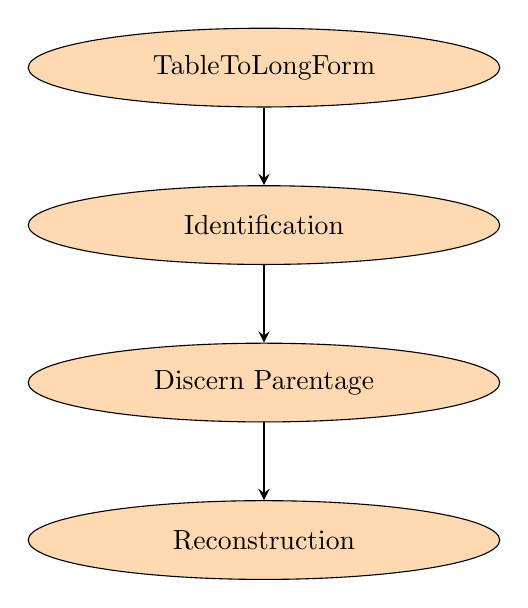
\begin{tikzpicture}[node distance=2cm]
\node (TTLFcall)[process]{TableToLongForm};
\node (Ident)[process, below of=TTLFcall]{Identification};
\node (Pare)[process, below of=Ident]{Discern Parentage};
\node (Recons)[process, below of=Pare]{Reconstruction};
\draw [arrow](TTLFcall) -- (Ident);
\draw [arrow](Ident) -- (Pare);
\draw [arrow](Pare) -- (Recons);
\end{tikzpicture}  
\caption{The basic workflow of TableToLongForm. There are 3 stages in
  the conversion process:}
\begin{enumerate}
\item Identification - identify where in the Table the data is found
  and where the accompanying labels are, while ignoring any extraneous
  information we do not want.
\item Parentage - understand the hierarchical structure (the
  \emph{parentage}) of the row and column labels.
\item Reconstruction - use the information from the first two stages
  to reconstruct the Table as a Dataframe.
\end{enumerate}
\end{figure}

\begin{figure}[!h]
  \centering
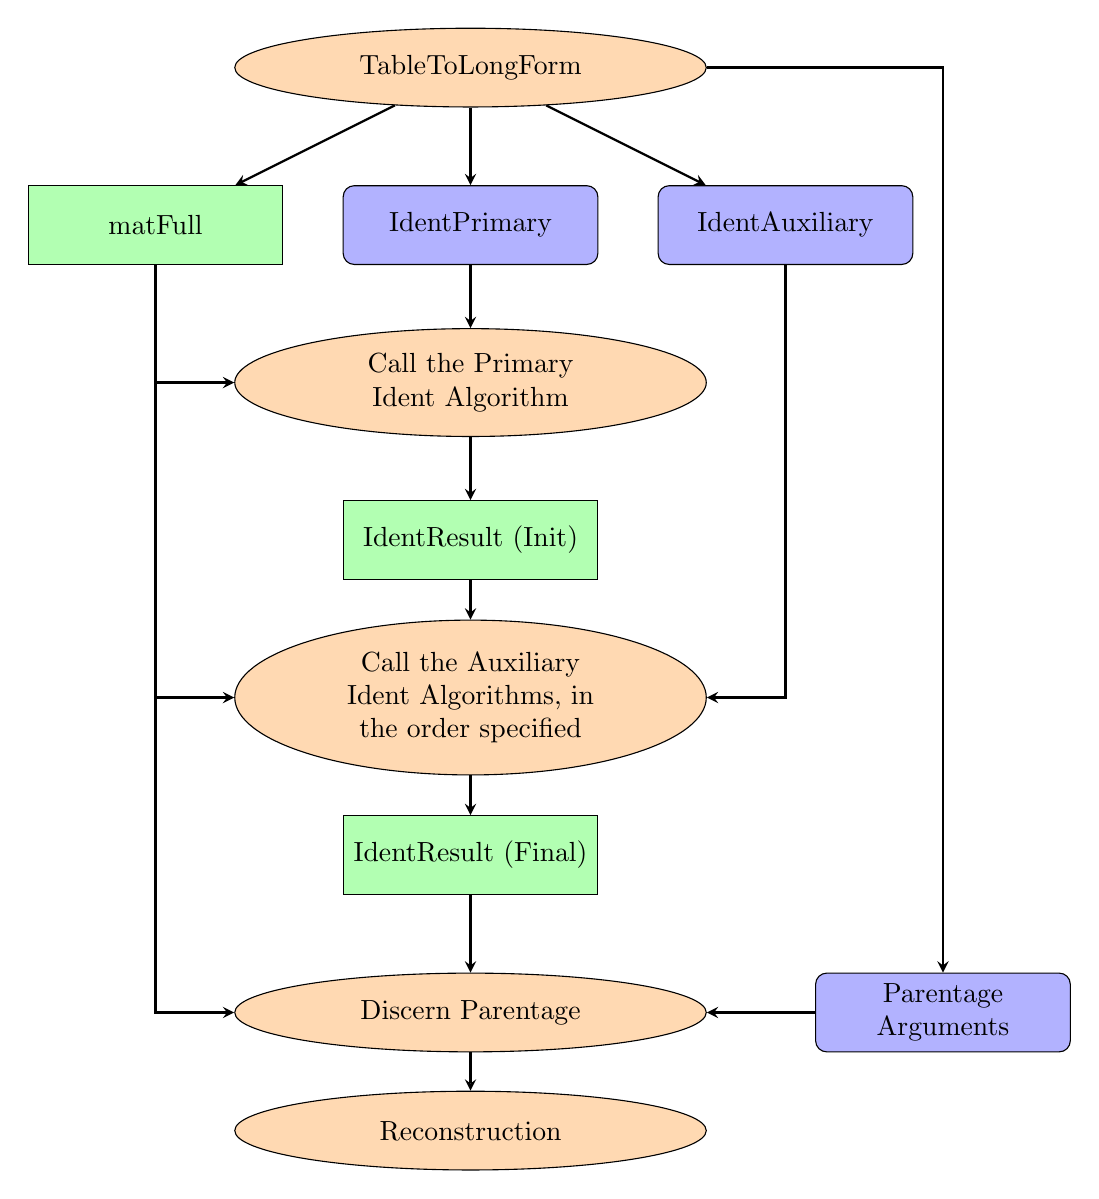
\begin{tikzpicture}[node distance=2cm]
\node (TTLFcall)[process]{TableToLongForm};
\node (IdentPrimary)[arg, below of=TTLFcall]{IdentPrimary};
\node (IdentAuxiliary)[arg, right of=IdentPrimary, xshift=2cm]{IdentAuxiliary};
\node (matFull)[vari, left of=IdentPrimary, xshift=-2cm]{matFull};
\draw [arrow](TTLFcall) -- (matFull);
\draw [arrow](TTLFcall) -- (IdentPrimary);
\draw [arrow](TTLFcall) -- (IdentAuxiliary);

\node (IdentPcall)[process, below of=IdentPrimary]{Call the Primary Ident Algorithm};
\draw [arrow](matFull) |- (IdentPcall);
\draw [arrow](IdentPrimary) -- (IdentPcall);

\node (IdentResulti)[vari, below of=IdentPcall]{IdentResult (Init)};
\draw [arrow](IdentPcall) -- (IdentResulti);

\node (IdentAcall)[process, below of=IdentResulti]{Call the Auxiliary Ident Algorithms, in the order specified};
\draw [arrow](matFull) |- (IdentAcall);
\draw [arrow](IdentAuxiliary) |- (IdentAcall);
\draw [arrow](IdentResulti) -- (IdentAcall);

\node (IdentResultii)[vari, below of=IdentAcall]{IdentResult (Final)};
\draw [arrow](IdentAcall) -- (IdentResultii);

\node (Pare)[process, below of=IdentResultii]{Discern Parentage};
\node (PareArgs)[arg, right of=Pare, xshift=4cm]{Parentage Arguments};
\node (Recons)[process, below of=Pare, yshift=0.5cm]{Reconstruction};
\draw [arrow](TTLFcall) -| (PareArgs);
\draw [arrow](PareArgs) -- (Pare);
\draw [arrow](matFull) |- (Pare);
\draw [arrow](IdentResultii) -- (Pare);
\draw [arrow](Pare) -- (Recons);
\end{tikzpicture}
\caption{We break down the Identification stage in more detail. The
  Table argument is referred to as matFull internally. The
  IdentPrimary and IdentAuxiliary arguments specify what algorithms
  will be called at the respective steps of the workflow.}
\end{figure}


\begin{figure}[!h]
  \centering
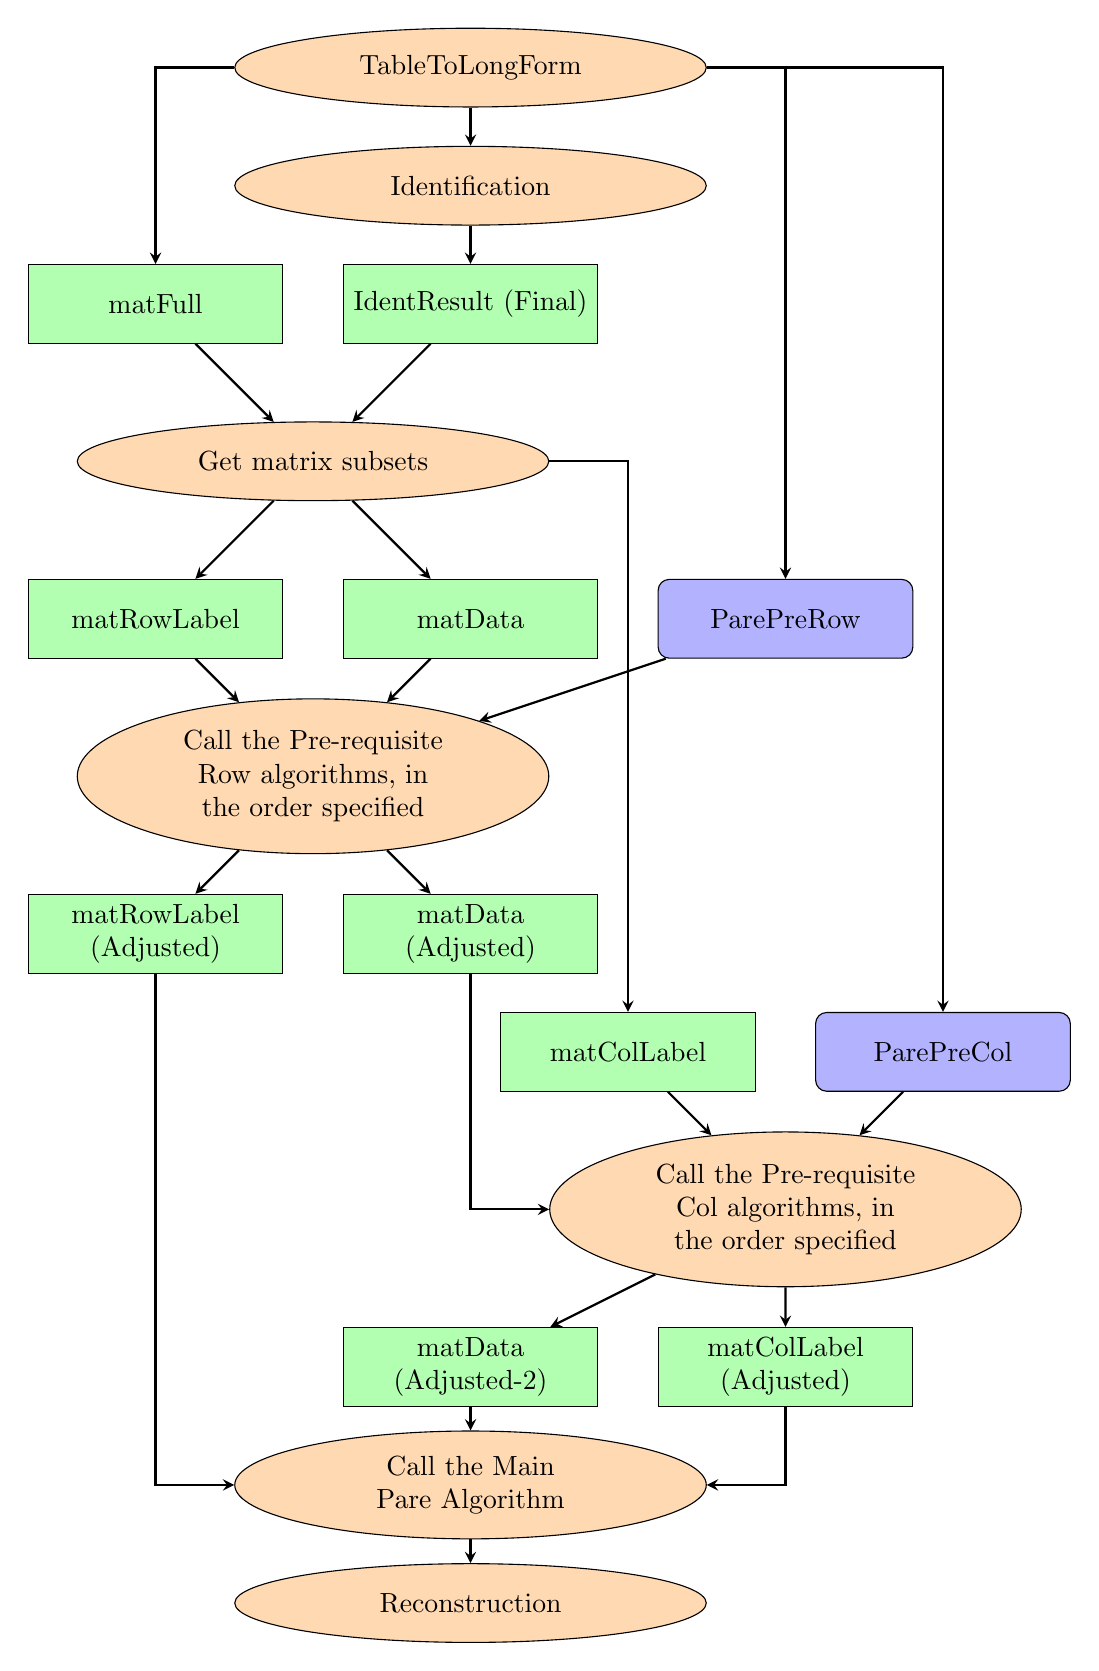
\begin{tikzpicture}[node distance=2cm]
\node (TTLFcall)[process]{TableToLongForm};
\node (Ident)[process, below of=TTLFcall, yshift=0.5cm]{Identification};
\draw [arrow](TTLFcall) -- (Ident);

\node (IdentResult)[vari, below of=Ident, yshift=0.5cm]{IdentResult (Final)};
\draw [arrow](Ident) -- (IdentResult);
\node (matFull)[vari, left of=IdentResult, xshift=-2cm]{matFull};
\draw [arrow](TTLFcall) -| (matFull);

\node (matGet)[process, below of=matFull, xshift=2cm]{Get matrix subsets};
\draw [arrow](matFull) -- (matGet);
\draw [arrow](IdentResult) -- (matGet);
\node (matData)[vari, below of=matGet, xshift=2cm]{matData};
\node (matRowLabel)[vari, left of=matData, xshift=-2cm]{matRowLabel};
\draw [arrow](matGet) -- (matData);
\draw [arrow](matGet) -- (matRowLabel);

\node (ParePreRow)[arg, right of=matData, xshift=2cm]{ParePreRow};
\draw [arrow](TTLFcall) -| (ParePreRow);

\node (ParePRcall)[process, below of=matData, xshift=-2cm]{Call the Pre-requisite Row algorithms, in the order specified};
\draw [arrow](matData) -- (ParePRcall);
\draw [arrow](matRowLabel) -- (ParePRcall);
\draw [arrow](ParePreRow) -- (ParePRcall);

\node (matDataii)[vari, below of=ParePRcall, xshift=2cm]{matData (Adjusted)};
\node (matRowLabelii)[vari, left of=matDataii, xshift=-2cm]{matRowLabel (Adjusted)};
\draw [arrow](ParePRcall) -- (matDataii);
\draw [arrow](ParePRcall) -- (matRowLabelii);

\node (ParePreCol)[arg, right of=matDataii, xshift=4cm, yshift=-1.5cm]{ParePreCol};
\draw [arrow](TTLFcall) -| (ParePreCol);
\node (matColLabel)[vari, left of=ParePreCol, xshift=-2cm]{matColLabel};
\draw [arrow](matGet) -| (matColLabel);

\node (ParePCcall)[process, below of=matColLabel, xshift=2cm]{Call the Pre-requisite Col algorithms, in the order specified};
\draw [arrow](matDataii) |- (ParePCcall);
\draw [arrow](matColLabel) -- (ParePCcall);
\draw [arrow](ParePreCol) -- (ParePCcall);

\node (matDataiii)[vari, below of=ParePCcall, xshift=-4cm]{matData (Adjusted-2)};
\node (matColLabelii)[vari, right of=matDataiii, xshift=2cm]{matColLabel (Adjusted)};
\draw [arrow](ParePCcall) -- (matDataiii);
\draw [arrow](ParePCcall) -- (matColLabelii);

\node (PareMcall)[process, below of=matDataiii, yshift=0.5cm]{Call the Main Pare Algorithm};
\draw [arrow](matDataiii) -- (PareMcall);
\draw [arrow](matRowLabelii) |- (PareMcall);
\draw [arrow](matColLabelii) |- (PareMcall);

\node (Recons)[process, below of=PareMcall, yshift=0.5cm]{Reconstruction};
\draw [arrow](PareMcall) -- (Recons);
\end{tikzpicture}
\caption{We break down the Discern Parentage stage in more detail. We
  use the IdentResult from the Identification stage to obtain subsets
  of matFull that correspond to just the labels or the data. We can
  then use these subsets to discern the parentage of the labels. The
  ParePreRow and ParePreCol arguments specify what algorithms will be
  called at the respective steps of the workflow, and they make
  adjustments to the matrix subsets so that the Main Parentage
  algorithm can function correctly.}
\end{figure}

\clearpage
\section{Registering a New Module}
This is done with a call to \verb|TTLFaliasAdd|, which has the
following arguments:
\begin{description}
\item[Type] e.g. IdentPrimary
\item[Fname] the name of the Function/Algorithm
\item[Falias] the alias for the Function/Algorithm, which is used for
  the call to \verb|TableToLongForm|
\item[Author] (optional) name of the author of the algorithm
\item[Description] (optional) a short description of the purpose of
  the algorithm
\end{description}

For example, the following is used to register the default Ident
Primary algorithm.
\begin{verbatim}
TTLFaliasAdd("IdentPrimary", "IdentbyMostCommonBoundary", "combound",
             "Base Algorithm", "Default IdentPrimary algorithm")
\end{verbatim}

The \verb|.R| file that contains the function(s) should also contain
this registration line. Then during an R session, one can load the
TableToLongForm package, then source the module's \verb|.R| file to
register the module's algorithm(s).

One can check if this is successful by then calling
\verb|TTLFaliasList|. The output with no additional modules is as
follows (line-breaks added):
\begin{verbatim}
> TTLFaliasList()
==Type: IdentPrimary==
Name: IdentbyMostCommonBoundary
Alias: combound
Author: Base Algorithm
Description: Default IdentPrimary algorithm

==Type: IdentAuxiliary==
Name: IdentbySequence
Alias: sequence
Author: Base Algorithm
Description: Search for fully numeric row labels (e.g. Years)
  that were misidentified as data

==Type: ParePreCol==
Name: ParePreColMismatch
Alias: mismatch
Author: Base Algorithm
Description: Correct for column labels not matched correctly
  over data (label in a different column to data)

Name: ParePreColMisaligned
Alias: misalign
Author: Base Algorithm
Description: Correct for column labels not aligned correctly over
  data (parents not positioned on the far-left, relative to their
  children in the row below)

Name: ParePreColMultirow
Alias: multirow
Author: Base Algorithm
Description: Merge long column labels that were physically split
  over multiple rows back into a single label
\end{verbatim}
If your new algorithms were successfully registered, they should
appear on this list, and the aliases for the new algorithms can be
used during a call to \verb|TableToLongForm|.

\end{document}